
\documentclass[review]{elsarticle}


\usepackage{lineno}%\usepackage[hyphens]{url}
\usepackage{url}
\usepackage{breakurl}
\usepackage{balance}

\usepackage{caption}
\usepackage{subcaption}

\usepackage{multirow}
\usepackage{booktabs}

\usepackage{xcolor}
\usepackage{soul}
\usepackage{comment}
\usepackage[colorinlistoftodos]{todonotes}
\usepackage{colortbl}


%\usepackage[ruled,vlined]{algorithm2e}
%\usepackage[ruled,vlined,linesnumbered,noresetcount]{algorithm2e}
\usepackage{algorithm}

\usepackage{algorithmic}

\usepackage{lscape}
\usepackage{algpseudocode}
\usepackage{tikz}
\usepackage{dirtree}
\newcommand\mybox[2][]{\tikz[overlay]\node[fill=blue!20,inner sep=2pt, anchor=text, rectangle, rounded corners=1mm,#1] {#2};\phantom{#2}}
\def\NoNumber#1{{\def\alglinenumber##1{}\State #1}\addtocounter{ALG@line}{-1}}

%\newcommand*\circled[1]{\tikz[baseline=(char.base)]{\node[shape=circle,fill=blue!20,draw,inner sep=1pt] (char) {#1};}}
%\newcommand*\circled[1]{\tikz[baseline=(char.base)]{\node[shape=circle,draw,inner sep=1pt] (char) {#1};}}

\renewcommand{\algorithmicforall}{\textbf{for each}}

\usepackage[acronym,nonumberlist,shortcuts,sanitize=none,nomain]{glossaries}
\makeglossaries
\usepackage[utf8]{inputenc}
\usepackage[english]{babel}
\usepackage{rotating}
\usepackage{lscape}
\usepackage{rotating}   
\usepackage{enumitem}
\usepackage{longtable}

\usepackage{makecell}
\usepackage{lmodern}
\usepackage{array}
\usepackage{enumerate}
\usepackage{times}



\usepackage[colorlinks=true, pdfstartview=FitV, linkcolor=blue, citecolor=blue, urlcolor=blue]{hyperref}


\journal{Information Science}

%%%%%%%%%%%%%%%%%%%%%%%
%% Elsevier bibliography styles
%%%%%%%%%%%%%%%%%%%%%%%
%% To change the style, put a % in front of the second line of the current style and
%% remove the % from the second line of the style you would like to use.
%%%%%%%%%%%%%%%%%%%%%%%

%% Numbered
%\bibliographystyle{model1-num-names}

%% Numbered without titles
%\bibliographystyle{model1a-num-names}

%% Harvard
%\bibliographystyle{model2-names.bst}\biboptions{authoryear}

%% Vancouver numbered
%\usepackage{numcompress}\bibliographystyle{model3-num-names}

%% Vancouver name/year
%\usepackage{numcompress}\bibliographystyle{model4-names}\biboptions{authoryear}

%% APA style
%\bibliographystyle{model5-names}\biboptions{authoryear}

%% AMA style
%\usepackage{numcompress}\bibliographystyle{model6-num-names}

%% `Elsevier LaTeX' style
%%%%%%%%%%%%%%%%%%%%%%%
\newcommand{\AlgoResetCount}{\renewcommand{\@ResetCounterIfNeeded}{\setcounter{AlgoLine}{0}}}
\newcommand{\AlgoNoResetCount}{\renewcommand{\@ResetCounterIfNeeded}{}}
\newcounter{AlgoSavedLineCount}
\newcommand{\AlgoSaveLineCount}{\setcounter{AlgoSavedLineCount}{\value{AlgoLine}}}
\newcommand{\AlgoRestoreLineCount}{\setcounter{AlgoLine}{\value{AlgoSavedLineCount}}}

\begin{document}

\begin{frontmatter}

\title{Detection and Classification of Sexual Content in Videos Using a Multimodal Model with Audio and Image Analysis }


\author[dir]{Luis Javier Garc\'ia Villalba\corref{cor1}}
\ead{javiergv@fdi.ucm.es}
\author[dir]{Carlos Quinto Huamán}
\ead{cquinto@ucm.es}
\author[dir]{Ana Lucila Sandoval Orozco}
\ead{asandoval@fdi.ucm.es}
\address[dir]{Group of Analysis, Security and Systems (GASS)\\
		Department of Software Engineering and Artificial Intelligence (DISIA)\\
		Faculty of Computer Science and Engineering, Office 431\\
		Universidad Complutense de Madrid (UCM)\\
		Calle Profesor Jos\'e Garc\'ia Santesmases 9, Ciudad Universitaria, 28040 Madrid, Spain}
\cortext[cor1]{Corresponding author}						

%\maketitle

\begin{abstract}

Tasks such as strategic decision making or budgeting are very important for companies to develop efficiently. For this reason, companies often turn to experts or to tools such as forecasting and scenario analysis in order to have all the possible information and to be prepared.
In this work, the insurance sector has been chosen, a sector where sales made through intermediaries (salespeople) are very common. The way in which the commercial discount offered by the intermediary affects his customers were studied, the different ways in which it can be applied and how the company can increase its profits through the sales requirements that it can impose on the intermediary in the contract.
In order to find a solution to this problem, a model has been created that estimates the results that the intermediary can obtain by following four different discount strategies: No discount, variable discount, progressive discount and maximum discount.
%Tareas como la toma de decisiones estratégicas o establecer presupuestos son muy importantes para que las empresas se desarrollen de forma eficiente. Por este motivo las empresas suelen recurrir a expertos o herramientas como la predicción de resultados y el análisis de escenarios para tener toda la información posible y poder prepararse.
%En este trabajo se ha elegido el sector asegurador, un sector donde es muy frecuente las ventas realizadas a través de mediadores (comerciales). Se ha estudiado como afecta el descuento comercial que ofrece el mediador a sus clientes, las distintas formas en las que puede aplicarlo y como la empresa puede aumentar sus beneficios mediante los requisitos de ventas que le puede poner al mediador en el contrato.
%Para encontrar la solución de este problema se ha realizado un modelo que estime los resultados que puede obtener el mediador siguiendo cuatro estrategias de descuento diferentes: Sin descuento, descuento variable, descuento progresivo y descuento máximo.


\end{abstract}

\begin{keyword}
Atom Extraction, Container Structure Analysis, Forensics Analysis, Multimedia Container, Social Media Detection, Supervised Classification Techniques, Video Forgery, Video Source Identification.
\end{keyword}

\end{frontmatter}
\newacronym{AAC}{AAC}{\textit{Advanced Audio Coding}}
\newacronym{AI}{AI}{\textit{Artificial Intelligence}}
\newacronym{ASCII}{ASCII}{\textit{American Standard Code for Information Interchange}}
\newacronym{ADC}{ADC}{\textit{Analog Digital Conversion}}
\newacronym{API}{API}{\textit{Application Programming Interface}}
\newacronym{AVI}{AVI}{\textit{Audio Interleave de Microsoft}}
\newacronym{CCD}{CCD}{\textit{Charge Coupled Device}}
\newacronym{CFA}{CFA}{\textit{Color Filter Array}}
\newacronym{CMOS}{CMOS}{\textit{Complementary Metal Oxide Semiconductor}}
\newacronym{CMY}{CMY}{\textit{Cyan-Magenta-Yellow}}
\newacronym{CYYM}{CYYM}{\textit{Cyan-Yellow-Yellow-Magenta}}
\newacronym{DBC}{DBC}{\textit{Decision Boundary Carving}}
\newacronym{DCT}{DCT}{\textit{Discrete Cosine Transform}}
\newacronym{DIP}{DIP}{\textit{Digital Image Processor}}
\newacronym{DSC}{DSC}{\textit{Digital Still Camera}}
\newacronym{DSP}{DSP}{\textit{Digital Signal Processor}}
\newacronym{EM}{EM}{\textit{Expectation-Maximization}}
\newacronym{EXIF}{EXIF}{\textit{Exchangeable Image File Format}}
\newacronym{FAR}{FAR}{\textit{False Acceptance Rate}}
\newacronym{FPN}{FPN}{\textit{Fixed Pattern Noise}}
\newacronym{GPS}{GPS}{\textit{Global Positioning System}}
\newacronym{GRGB}{GRGB}{\textit{Green-Red-Green-Blue}}
\newacronym{IFD}{IFD}{\textit{Image File Directory}}
\newacronym{IID}{IID}{\textit{Independent and Identically Distributed random variable}}
\newacronym{IQM}{IQM}{\textit{Image Quality Metrics}}
\newacronym{IP}{IP}{\textit{ Internet Protocol}}
\newacronym{ISO}{ISO}{\textit{International Organization for Standardization}}
\newacronym{IEC}{IEC}{\textit{International Electrotechnical Commission}}
\newacronym{ITU}{ITU}{\textit{International Telecommunication Union}}
\newacronym{JPEG}{JPEG}{\textit{Joint Photographic Experts Group}}
\newacronym{MAP}{MAP}{\textit{Maximum A-Posteriori Probability}}
\newacronym{ML}{ML}{\textit{Machine Learning}}

\newacronym{MOS}{MOS}{\textit{Metal Oxide Semiconductor}}
\newacronym{MPEG}{MPEG}{\textit{Moving Picture Experts Group}}
\newacronym{AI}{AI}{\textit{Artificial Intelligence}}
\newacronym{RAM}{RAM}{\textit{Random Access Memory}}
\newacronym{IP}{IP}{\textit{Internet Protocol}}
\newacronym{MKV}{MKV}{\textit{Matroska}}
\newacronym{PDA}{PDA}{\textit{Personal Digital Assistant}}
\newacronym{PCE}{PCE}{\textit{Peak to Correlation Energy}}
\newacronym{PCA}{PCA}{\textit{Principal Component Analysis}}
\newacronym{PNU}{PNU}{\textit{Pixel Non-Uniformity}}
\newacronym{PRNU}{PRNU}{\textit{Photo Response Non Uniformity}}
\newacronym{QMF}{QMF}{\textit{Separable Quadrate Mirror Filters}}
\newacronym{RBF}{RBF}{\textit{Radial Basis Function}}
\newacronym{RGB}{RGB}{\textit{Red-Green-Blue}}
\newacronym{RAM}{RAM}{\textit{Random Access Memory}}
\newacronym{RGBE}{RGBE}{\textit{Red-Green-Blue-Emerland}}
\newacronym{ROI}{ROI}{\textit{Region Of Interest}}
\newacronym{SFFS}{SFFS}{\textit{Sequential Forward Featured Selection}}
\newacronym{SFS}{SFS}{\textit{Sequential Floating Search}}
\newacronym{SPN}{SPN}{\textit{Sensor Pattern Noise}}
\newacronym{SVM}{SVM}{\textit{Support Vector Machine}}
\newacronym{SMOTE}{SMOTE}{\textit{Syntethic Minority OverSampling}}
\newacronym{TSNE}{TSNE}{\textit{T-distributed Stochastic Neighbor Embedding}}

\newacronym{TIFF}{TIFF}{\textit{Tagged Image File Format}}
\newacronym{XMP}{XMP}{\textit{eXtensible Metadata Platform}}
\newacronym{RAT}{RAT}{\textit{Radon Transform}}
\newacronym{PSD}{PSD}{\textit{Photoshop Data file}}
\newacronym{MAE}{MAE}{\textit{Mean Absolute Error}}
\newacronym{MSE}{MSE}{\textit{Mean Square Error}}
\newacronym{VEDRS}{VEDRS}{\textit{Video Event Data Recorders}}
\newacronym{XML}{XML}{\textit{Extensible Markup Language}}

\newacronym{TP}{TP}{\textit{True Positives}}
\newacronym{FN}{FN}{\textit{False Negatives}}
\newacronym{TN}{TN}{\textit{True Negatives}}
\newacronym{FP}{FP}{\textit{False Positives}}

\newacronym{LR}{LR}{\textit{Logistic  Regression}}
\newacronym{DT}{DT}{\textit{Decision Tree}}
\newacronym{LDA}{LDA}{\textit{Linear  Discriminant  Analysis}}
\newacronym{GNB}{GNB}{\textit{Gaussian  Naive  Bayes}}
\newacronym{KNN}{KNN}{\textit{KNeighbors}}
\newacronym{RF}{RF}{\textit{Random Forest}}
\newacronym{GBC}{GBC}{\textit{Gradient   Boosting   Classifier}}
\newacronym{XGB}{XGB}{\textit{Extreme Gradient Boosting}}




\section{Introduction}

Companies such as Mapfre, Liberty Seguros Génesis or Allianz are dedicated to the sale of insurance. Allianz defines insurance as a contract \cite{allianz2023seguros}, are contracts drawn up in good faith in which they insurer agrees to pay the insured a certain benefit, an income or a capital, in the event that a future event foreseen in the policy occurs, in exchange for the insured paying the premium.
There are numerous insurance categories to protect against a wide range of potential future events. However, this work utilises the data presented in the 2021 Sector Report \cite{dgsfp2022informe} in table 1 of the annex, which includes non-life insurance.
The definition of these insurances from \cite{mapfre2023diccionario} is:
%Empresas como Mapfre, Liberty Seguros Génesis o Allianz se dedican a la venta de seguros que según (Allianz, 2023) son contratos elaborados de buena fe en los que se comprometen a satisfacer al asegurado una prestación determinada, una renta o un capital, en el caso de que se produzca un evento futuro previsto en la póliza, a cambio de que el asegurado pague la prima.Hay muchas ramas de seguros diferentes para cubrir todo tipo de eventos futuros, sin embargo, en este trabajo se han utilizado los encontrados en el Informe del sector 2021 (DGSFP, 2022) en la tabla1 del anexo, que recoge los seguros de no vida.La definición de estos seguros de (Mapfre, 2023) es:

Accident: In general terms, an eventual event or action that results in involuntary damage to people or things. For insurance purposes, an act or fact that results from a violent, sudden, external and involuntary cause that causes damage to people or things. It is also synonymous with loss or breakdown.
%Accidente: En términos generales, suceso eventual o acción del que resulta un daño involuntario para las personas o las cosas. A los efectos del seguro, acto o hecho que deriva de una causa violenta, súbita, externa e involuntaria que produce daños en las personas o en las cosas. Es también sinónimo de siniestro o avería.

Illness: In general, any involuntary alteration of health diagnosed by a doctor legally authorised to practise. For the purposes of coverage in some insurance policies (e.g. Health, Personal Accident, Dental, etc.), by way of example and not limitation, it is usually specified that sterility, weight loss treatments, sleep or rest cures, psychological treatments, interventions and/or treatments for aesthetic reasons, congenital defects or ailments, alcoholism and drug addiction are not considered illnesses. It can be synonymous with injury.
%Enfermedad: Con carácter general, es toda alteración involuntaria de la salud cuyo diagnóstico sea efectuado por un médico legalmente autorizado para ejercer. A los efectos de la cobertura en algunos seguros (p. ej., Salud, Accidentes personales, Dental,…), a título meramente enunciativo y no limitativo, suele especificarse que no se consideran enfermedad la esterilidad, los tratamientos para adelgazar, las curas de sueño o reposo, los tratamientos psicológicos, las intervenciones y/o tratamientos por razones estéticas, los defectos o dolencias congénitas, el alcoholismo y las toxicomanías. Puede ser sinónimo de lesión.

Health care: Set of benefits derived from medical-hospital treatment provided to people with illness or injuries due to accidents of any kind.
%Asistencia sanitaria: Conjunto de prestaciones derivadas del tratamiento médico-hospitalario efectuado a personas con enfermedad o lesionadas a causa de accidentes de cualquier clase.

Civil liability: In general, it is the obligation of a person to repair the damages and losses caused to another as a result of an action or omission, either their own or that of a third party for which they are responsible, in which there has been some type of fault or negligence.
%Responsabilidad civil: En general, es la obligación que tiene una persona de reparar los daños y perjuicios producidos a otra a consecuencia de una acción u omisión, propia o de tercero por el que deba responderse, en que haya habido algún tipo de culpa o negligencia.

Legal defense: Insurance coverage by which the insurer assumes the claim and defense for damages of the insured.
%Defensa jurídica: Cobertura de seguro por la cual la aseguradora asume la reclamación y defensa por daños y perjuicios del asegurado.

Travel assistance: Type of insurance whose purpose is to provide assistance to the insured who may find themselves in a difficult and/or emergency situation during a trip. The main characteristic of this type of insurance is that it is a service provision insurance as opposed to typical compensatory insurance: the provision of assistance services that resolve difficult and/or emergency situations for the insured takes precedence over financial compensation.
%Asistencia viajes: Modalidad de seguro cuyo objeto es la prestación de ayuda a los asegurados que puedan hallarse en situación de dificultad y/o emergencia en el transcurso de un viaje. La característica principal de este tipo de seguros es que es un seguro de prestación de servicios frente al típico seguro compensatorio: prima la prestación de servicios de asistencia que resuelvan situaciones de dificultad y/o emergencia de los asegurados sobre las compensaciones económicas.

Death: Synonym for burial insurance. Type of insurance under which, in the event of the death of the insured, the compensation provided for in the contract is given to his/her relatives and/or the services necessary for the burial ceremony are provided (funeral services).
%Decesos: Sinónimo de seguro de enterramiento. Modalidad de seguro en virtud de la cual, en caso de fallecimiento del asegurado, se entrega a sus familiares la indemnización prevista en el contrato y/o se prestan los servicios necesarios para el acto de sepelio (pompas fúnebres).

Multi-risk: This is the type of insurance that guarantees the most important risks to which the goods to be covered are subject in a single contract. It is also called combined insurance. Multi-risk insurance is classified as Simple and Industrial. The basic types of Simple Multi-risk are: Home Insurance, which aims to provide financial security to the tenant or owner against the economic consequences that may arise from damage affecting their property or civil liabilities that may be incumbent upon them; Community Insurance, with a structure similar to Home Insurance, but referring to real estate, generally under a community of co-owners; Commercial (retail) and Office Insurance, which aims to guarantee the insured compensation for losses due to economic damages arising from the main risks affecting the market sector to which it is directed. Industrial Multi-risk is aimed primarily at specific sectors that have high insured sums and at establishments where some type of industrial activity or storage of high insured sums is carried out. Although it can also cover non-manufacturing activities such as schools, hospitals, supermarkets, etc.
%Multirriesgo: Es aquel por el que en un solo contrato se garantizan los riesgos más importantes a los que están sujetos los bienes objeto de cobertura. También se denomina seguro combinado. Los seguros multirriesgo se clasifican en Sencillos e Industriales. Las modalidades básicas de Multirriesgos Sencillos son: Seguro de Hogar, que tiene por objeto proporcionar una seguridad financiera al inquilino o propietario ante las consecuencias económicas que puedan derivarse de un daño que afecte a sus bienes o de las responsabilidades civiles que le puedan incumbir; Seguro de Comunidades, con una estructura similar al Seguro del Hogar, pero referido a inmuebles, generalmente en régimen de comunidad de copropietarios; Seguros de Comercios (minoristas) y Oficinas, que tiene como objeto garantizar al asegurado la compensación de las pérdidas por perjuicios económicos derivados de los principales riesgos que afectan al sector del mercado al cual se dirige. Los Multirriesgos Industriales van dirigidos fundamentalmente a sectores específicos que presentan sumas aseguradas elevadas y a establecimientos donde se realiza algún tipo de actividad industrial o almacenamientos de elevada suma asegurada. Aunque también puede recoger actividades no fabriles como colegios, hospitales, supermercados, etc

Agricultural insurance: Coverage system that exists in Spain to protect against certain risks, especially climatic risks, the most important agricultural crops in the country and certain species of the national livestock. Each year the Administration itself establishes a plan in which protected crops and animals are established, subsidies for premiums, coverage, etc.
%Seguros agrarios: Sistema de cobertura que existe en España para proteger frente a determinados riesgos, especialmente climatológicos, los cultivos agrícolas más significativos del país y ciertas especies de la cabaña nacional. Cada año la propia Administración establece un plan en el que se establecen cultivos y animales protegidos, subvenciones a las primas, coberturas, etc.

In this sector, in addition to the most popular distribution channels such as the company's own offices, the Internet and the telephone, many insurance sales are made through another means, linked agents or mediators. In Spain, there were 56,420 exclusive agents operating in 2020. \cite{dgsfp2022informe}.
A linked agent or mediator is a company-employed professional who communicates with clients, provides advise and is responsible for managing contracts.Therefore Mastery of communication, attention, empathy and customer care skills is essential for offering a quality service and achieving high sales volumes.
%En este sector además de los canales de distribución más populares como las oficinas de la propia empresa, internet y el teléfono, muchas de las ventas de los seguros se realizan a través de otro medio, los agentes vinculados o mediadores, llegando a operar 56.420 agentes exclusivos en España en el año 2020 (DGSFP, 2022).
%Un agente vinculado o mediador es un profesional que trabaja para la empresa y se comunica con los clientes, les asesora y se encarga de la gestión del contrato, por lo que es imprescindible dominar habilidades como la comunicación, atención, empatía o la cercanía para ofrecer un servicio de calidad a la par que un gran volumen de ventas.

Furthermore, it is common practice for companies to set minimum objectives or requirements in contracts, depending on their policies. Failure to meet these requirements may result in the non-renewal of your contract or a reduction in salary. However, meeting these objectives could result in bonuses.
Ultimately, the mediator must achieve set targets in a challenging sector where sales volumes can be influenced by numerous variables and there is a significant risk of not meeting targets. It is therefore common practice for mediators to offer discounts to clients in order to increase sales and mitigate risk.
%Además, es muy común dependiendo de las políticas de cada empresa, que se fijen en los contratos unos objetivos o requisitos mínimos. No cumplirlos podría implicar la no renovación de su contrato o recibir un sueldo menor. Mientras que al cumplirlos podría lograr bonificaciones.
%Al final el mediador tiene la necesidad de alcanzar los objetivos en un sector muy duro en el que el volumen de ventas puede depender de muchos factores y hay un riesgo alto de no cumplir los objetivos. Por este motivo los mediadores se ven en la necesidad de ofrecer descuentos a los clientes para aumentar sus ventas y reducir el riesgo.

This discount is applied to the commission received by the brokers for the sale. The commission is the percentage of the premium that the broker receives in exchange for their services, which include sales and advisory activities. As with the minimum requirements, the commission may vary depending on the company in question. In this role, the commission is a fixed amount per product.
The company will determine the maximum discount that the broker is permitted to apply. Given that the discount is applied to the commission, the maximum discount that a broker can offer will be equal to their commission.

%Este descuento se aplica sobre la comisión que reciben los mediadores por la venta. La comisión es el porcentaje de la prima que recibe el mediador por la realización de los servicios de venta y asesoramiento. Igual que con los requisitos mínimos, dependiendo de cada empresa la comisión puede ser diferente. En este trabajo la comisión es fija para cada producto.
%La empresa fijará el máximo descuento que puede aplicar el mediador y como en este trabajo el descuento se aplica sobre la comisión, el máximo descuento que podrá ofrecer un mediador será igual a su comisión.

It should be noted that the pure premium received by the company remains constant regardless of the application of the discount. Based on these ideas, the objective of this study is to predict the results that the mediator can obtain based on the discount offered to its clients. Sales prediction studies are of great importance and are carried out in most companies regardless of the sector. They facilitate tasks such as strategic planning, budgets or inventory.
%Nótese que de esta manera la prima pura que recibe la empresa no varía con la aplicación del descuento.
%Sobre la base de estas ideas, el trabajo tiene como objetivo predecir los resultados que puede obtener el mediador en función del descuento que ofrezca a sus clientes.
%Los estudios sobre la predicción de ventas son muy importantes y se realizan en la mayoría de las empresas independientemente del sector. Facilitan labores como la planificación estratégica, los presupuestos o el inventario.

Several different simulations will be generated, changing in each one the commercial discount strategy that the mediator offers to its clients.
The strategies chosen for the work are:
%Se generarán varias simulaciones diferentes cambiando en cada una la estrategia del descuento comercial que el mediador ofrece a sus clientes.
%Las estrategias elegidas para el trabajo son:

\begin{enumerate}
    \item No Discount. Never offer a discount to clients regardless of their results or needs.%Sin descuento. Nunca ofrece un descuento a los clientes sin importar los resultados obtenidos ni sus necesidades.
    \item Maximum Discount: Offer all your customers the same discount until you reach your goals. Once you meet the minimum requirements, you no longer offer any discounts to customers.%Descuento máximo: Ofrece a todos sus clientes el mismo descuento hasta que consigue sus objetivos. Una vez que cumple los requisitos mínimos ya no ofrece ningún descuento a los clientes.
    \item Variable discount. The discount offered by the broker is random from 0 to the maximum that can be offered per contract.%Descuento variable. El descuento ofrecido por el mediador es aleatorio desde 0 hasta el máximo que puede ofrecer por contrato.
    \item Progressive discount. The broker first focuses on meeting the minimum requirements and offers the maximum discount. But as the broker approaches the target, the broker reduces the discount, applied progressively, to increase the commission he receives. %Descuento progresivo. El mediador primero centra sus esfuerzos en cumplir los requisitos mínimos y ofrece el máximo descuento. Pero según se va acercando al objetivo el mediador reduce el descuento, aplicado progresivamente, para aumentar la comisión que recibe.
\end{enumerate}

The results of the different strategies will allow:
\begin{enumerate}
    \item Analyze how the use of a commercial discount affects the success of the contracting process (and therefore the volume of contracted premium). See which strategy maximizes the probability of meeting the conditions (minimum requirements) of number of sales and income that the company may impose on the intermediary.
% Analizar como el uso de un descuento comercial afecta al éxito en el proceso de contratación (y por ende en el volumen de prima contratada). Ver cuál es la estrategia que maximiza las probabilidades de cumplir las condiciones (requisitos mínimos) de número de ventas e ingresos que le pueda imponer la empresa al mediador.
    \item Study how, depending on the values defined in the parameters (contracted premiums, minimum number of policies), the mediator may be forced to systematically offer the discount or never apply it.
%Estudiar cómo en función de los valores que se definan en los parámetros (primas contratadas, número mínimo de pólizas), el mediador se puede ver obligado a ofrecer sistemáticamente el descuento o a no aplicarlo nunca.
\end{enumerate}


Study how, depending on the values defined in the parameters (contracted premiums, minimum number of policies), the mediator may be forced to systematically offer the discount or never apply it.
%Estudiar cómo en función de los valores que se definan en los parámetros (primas contratadas, número mínimo de pólizas), el mediador se puede ver obligado a ofrecer sistemáticamente el descuento o a no aplicarlo nunca.



%El trabajo está estructurado en 6 secciones, siendo la primera la presente introducción. En la sección 2 se describe brevemente algunos conceptos sobre vídeos digitales. La sección 3 estudia las técnicas de análisis forense en vídeos y su interacción con el aprendizaje automático. En la sección 4 se describe la técnica propuesta. En la sección 5 se decribe los experimentos y resultados. Por último, en la sección 6 se presentan las conclusiones del presente trabajo.


\section{Methodology}

This section outlines the methodology employed during the development of the work, together with the theoretical foundations upon which it is based.
The following tasks were undertaken in the course of this research: the development of the model, the generation of cases and simulations, and the analysis of results.
%En este apartado se encuentra el procedimiento seguido durante el desarrollo del trabajo, así como sus fundamentos teóricos.En el trabajo se han realizado las siguientes tareas: desarrollo del modelo, generación de casos y simulación, y análisis de resultados.

\subsection{Model development}

In order to achieve this objective, a mathematical model has been developed. This can be defined as a simplified representation of reality which facilitates the negotiation of policies between a broker and their clients until the broker's working hours have elapsed.
In order to ensure that the simulation of the model is as close to reality as possible, a parametric model has been employed, comprising the broker's portfolio of policies and the variables that define the behaviour of each type of product. The aforementioned variables are frequency, premium, commission, probability of contracting, effort, and commercial discount.
%Con este objetivo en mente se ha realizado un modelo “matemático”, es decir, una forma simplificada de aproximarse a la realidad, que realice el proceso de negociación de pólizas de un mediador con sus clientes hasta que el mediador se quede sin horas de trabajo.Para conseguir que la simulación del modelo sea lo más parecida a la realidad se ha utilizado un modelo paramétrico, formado por la cartera de pólizas del medidor y las variables que definen el comportamiento de cada tipo de producto. Estas variables son frecuencia, prima, comisión, probabilidad de contratación y esfuerzo y el descuento comercial.


\textbf{Frequency}: Value between 0 and 100 that indicates the probability that negotiation will occur for the sale of each type of product.
%Frecuencia: Valor entre 0 y 100 que indica la probabilidad de que se produzca la negociación para la venta de cada tipo de producto.

\textbf{Insurance premium}: Average premium of the insurance policy. The concept of "insurance premium" refers to the price that the insurer pays to the insurer for the insurance contract.
%Prima de seguro: Prima media de la póliza. El concepto de prima de seguro se refiere al precio que el asegurador paga a la aseguradora por el contrato del seguro.

\textbf{Probability of contracting}: Value between 0 and 1, which indicates the probability that the mediator will be able to sell the policy.
%Probabilidad de contratación: Valor entre 0 y 1, que indica la probabilidad de que el mediador consiga vender la póliza.

\textbf{Duration}: Average hours that the mediator spends on the negotiations of each policy.
%Duración: Promedio de horas que el mediador dedica en las negociaciones de cada póliza.

\textbf{Commission}: Value between 0 and 1 that indicates the percentage of commission that the broker receives for the sale of each policy.
%Comisión: Valor entre 0 y 1 que indica el porcentaje de comisión que recibe el mediador por la venta de cada póliza.

\textbf{Discount}: Value between 0 and 100 that indicates the maximum value that the broker can offer regardless of the strategy followed.
%Descuento: Valor entre 0 y 100 que indica el máximo valor que el mediador puede ofrecer independientemente de la estrategia que se siga.

In addition to the product portfolio, the model has three other variables that affect consumer behavior: hours, policy objective and premium.
%Además de la cartera de productos el modelo tiene otras tres variables que afectan al comportamiento del consumidor, horas, objetivo de pólizas y prima.

\textbf{Hours}: Total number of hours worked by the mediator. For example, for a monthly study 160 working hours can be established, for a quarterly study 480 hours or for an annual study 1920 hours.
%Horas: Número de horas total que trabaja el mediador. Por ejemplo, para un estudio mensual se pueden establecer 160 horas laborales, trimestral 480 horas o anual 1920 horas.

\textbf{Policy target}: Number of policies that the company sets as a target for the mediator in its contract.

\textbf{Premium target}: Monetary amount in euros that the company sets as a target for the mediator in its contract.
%Objetivo pólizas: Numero de pólizas que la empresa le pone al mediador como objetivo en su contrato. Objetivo prima: Cantidad monetaria en euros que la empresa le pone al mediador como objetivo en su contrato.

Understanding the variables that make up each type of product, the following explains in more detail their characteristics, the theoretical basis that has been carried out and the relationships between the variables if they exist.
%Comprendiendo cuales son las variables de las que está formado cada tipo de producto, a continuación, se explican más en detalle sus características, cuál es el fundamento teórico que se ha realizado y las relaciones entre las variables en caso de que existan.

FREQUENCY

To determine what type of product each client wants, each product has an associated frequency or probability. Based on the frequency of each product, the order of sale of the policies is randomly generated for each sample.
The annual report of the insurance market \cite{dgsfp2022informe} has been taken as a reference, where the total volume of production in the non-life branches with insurance agents linked to individuals is found. This table shows the types of insurance with the highest production and those are the ones with the highest frequency.
%Para determinar qué tipo de producto quiere cada cliente, cada producto tieneasociada una frecuencia o probabilidad. En función de la frecuencia de cada producto de manera aleatoria se genera el orden de venta de las pólizas para cada muestra.Se ha tomado como referencia el informe anual del mercado asegurador (DGSFP, 2022) donde se encuentra el volumen total de producción en ramos no vida con agentes de seguros vinculados personas físicas. En esta tabla aparecen los tipos de seguros con mayor producción y esos son los que tienen una mayor frecuencia.

PREMIUM OF EACH PRODUCT

The premium of an insurance policy does not have a fixed price, it can vary according to an infinite number of factors such as: the coverage that the client needs, age, sex, history, territory, etc. Therefore, the premium is a random variable and the Weibull distribution has been used to define its behaviour.
According to the book of probability and statistics (Walpole, R. E, 2012): “The Weibull distribution is a distribution introduced by the physicist Waloddi Weibull in 1939 that together with current technology allows engineers to design many complicated systems whose operation and safety depend on the reliability of the various components that make up the systems”.
%La prima de una póliza de seguros no tiene un precio fijo, puede variar según una infinidad de factores como: la cobertura que necesite el cliente, la edad, el sexo, historial, territorio, etc. Por lo tanto, la prima es una variable aleatoria y para definir su comportamiento se ha utilizado la distribución Weibull.Tomando como referencia el libro de probabilidad y estadística (Walpole, R. E, 2012): “la distribución Weibull es una distribución introducida por el físico Waloddi Weibull en 1939 que junto con la tecnología actual permite que los ingenieros diseñen muchos sistemas complicados cuya operación y seguridad dependen de la confiabilidad de los diversos componentes que conforman los sistemas”

The reason why the Weibull distribution has been chosen over other more commonly used distributions, such as the Normal distribution, the Poisson distribution or the Student t, is due to the various applications found of this distribution in the insurance sector such as: modeling the severity of claims \cite{hamza2022weibull} the analysis of loss distributions in the sector \cite{ahmad2020modeling} or value-risk estimates \cite{gebizlioglu2011comparison}.
%El motivo por el que se ha elegido la distribución Weibull antes que otras distribuciones más utilizadas, como las distribución Normal, la distribución de Poisson o la t de Student, es debido a las diversas aplicaciones encontradas de esta distribución en el sector asegurador como: el modelado de la gravedad de las reclamaciones (Hamza, 2022), el análisis de distribuciones de perdidas en el sector (Ahmad, 2020) o estimaciones de valor- riesgo (Gebizlioglu, 2011)
\begin{figure}[h]
%\begin{minipage}[h]{9cm}
\centering
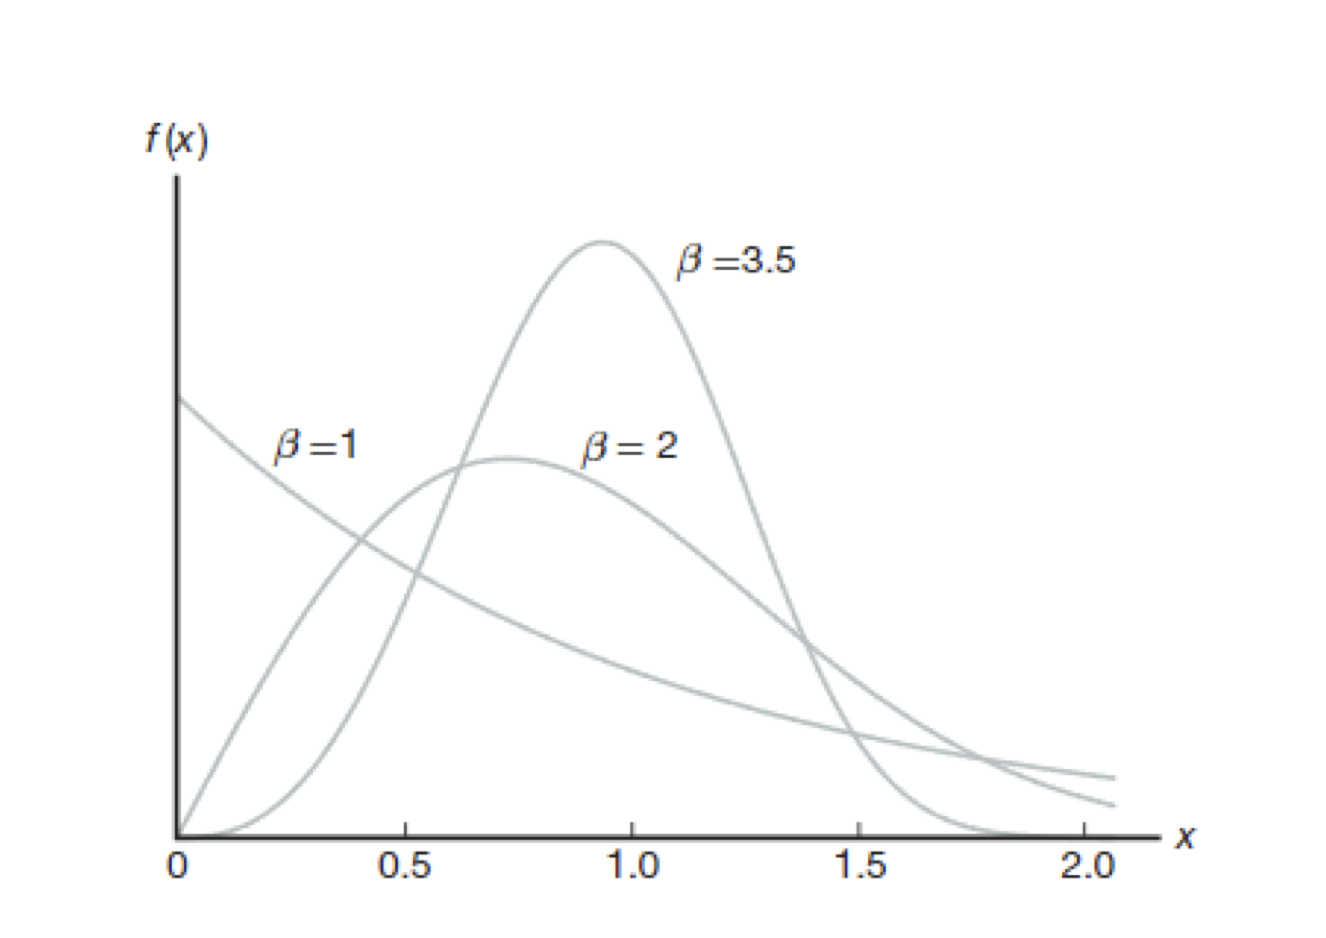
\includegraphics[width=\linewidth]{images/b1.png}
\caption{\label{fig2}Weibull Distribution (Alpha = 1)
technique.} 
%\end{minipage}
\end{figure}
PROBABILITY OF CONTRACTING

In the process of negotiating with a client, two events can occur: the broker manages to sell the policy (success) or he does not sell the policy (failure).
In order to determine the result of this experiment in each case, it is necessary to calculate the probability of each event. This probability depends on the premium of the policy being negotiated and the discount applied by the broker.
%En el proceso de negociación con un cliente se pueden producir dos eventos: que el mediador consiga vender la póliza (éxito) o que no venda la póliza (fracaso).Para determinar el resultado de este experimento en cada caso es necesario calcular la probabilidad de cada evento. Esta probabilidad depende de la prima de la póliza que este en negociación y del descuento que el mediador aplique.

Therefore, to generate the negotiation results it is necessary to define the probability of contracting the policies and its relationship with the discount.
The relationship between of a discount on prices and the probability of sale is very complex and as Alford \cite{alford2002effects} introduces, the way in which a discount affects the probability of purchase is determined by many factors, the consumers' perception of the value of the offer, the benefits of the consumers of the additional search or search intention and the intention to buy. There are also many studies that show how the same discount works differently depending on the type of store or product, the familiarity with the brand and the consistency and distinctiveness of the advertising.
%Por lo tanto, para generar los resultados de la negociación es necesario definir la probabilidad de contratación de las pólizas y su relación con el descuento. La relación de un descuento con los precios y la probabilidad de venta es muy compleja y como introduce Alford (2002) la manera en que un descuento afecta a la probabilidad de compra viene determinado por muchos factores, la percepción de los consumidores del valor de la oferta, los beneficios de los consumidores de la búsqueda adicional o la intención de búsqueda y la intención de compra. También hay muchos estudios que demuestran cómo un mismo descuento funciona de manera diferente dependiendo del tipo de tienda o producto, la familiaridad con la marca y la consistencia y el carácter distintivo de la publicidad.


Because of this and the lack of historical data, the way in which the average probability of contracting for each product has been established is subjective.
On the other hand, to establish how the probability of contracting is related to both the discount offered and the premium, Campbell \cite{campbell1990framing} explains the consumer's perception of the discount as an incentive to purchase. A 5\%  discount may be too small in some cases to be considered an incentive. And if, on the contrary, we offer a discount that is too large, this may be suspicious for some consumers and they will not make the purchase.
% Debido a esto y al no disponer de datos históricos, la manera en la que se ha fijado la probabilidad de contratación media de cada producto es subjetiva. Por otro lado, para establecer como se relaciona la probabilidad de contratación tanto con el descuento ofrecido como con la prima, Campbell (1990) explica la percepción que tiene el consumidor del descuento como un incentivo a la compra. Un descuento del 5% puede ser muy pequeño en algunos casos para ser considerado un incentivo. Y si al contrario ofrecemos un descuento demasiado grande este puede ser sospechoso para algunos consumidores y no realizarán la compra.

The discount will be an incentive to purchase the policy and will directly increase the probability of contracting it. However, the probability of contracting it decreases when the price moves away from the average value of the policy.
To calculate the probability of contracting it for each sample with respect to the average premium for the type of product, the following function has been used:
%El descuento será un incentivo para la compra de la póliza y aumentará la probabilidad de contratación directamente. Sin embargo, la probabilidad de contratación disminuye cuando el precio se aleja del valor medio de la póliza. Para calcular la probabilidad de contratación de cada muestra respecto a la prima media del tipo de producto se ha utilizado la siguiente función:

\begin{equation}
    w = (1 - \frac{|y - \Bar{y}|}{\Bar{y}} ) \times \Bar{w}
\end{equation}
\begin{itemize}
    \item w : hiring probability
    \item y : insurance premium
    \item \Bar{y}: average insurance premium x
    \item \Bar{w}: Average probability of insurance contract x
\end{itemize}

DURATION

This represents the difficulty of negotiating the policy and the time the broker spends on the policy. It is directly related to the policy premium, so it increases when the premium moves away from the average value.
%Representa la dificultad de la negociación de la póliza y el tiempo que el mediador dedica en la póliza. Está relacionado directamente con la prima de la póliza de manera que aumenta cuando la prima se aleja del valor medio.
\begin{equation}
    z = (1 + \frac{|y - \Bar{y}|}{\Bar{y}} ) \times \Bar{z}
\end{equation}

Z : Insurance duration
Z/ : Average insurance duration

COMMISSION, DISCOUNT, MINIMUM OBJECTIVES AND HOURS

These variables depend either on the decision of the company or the mediator.
Their values can be modified to study various scenarios and analyze the most appropriate strategy to achieve the objectives.
%Estas variables dependen o bien de la decisión de la empresa o del mediador. Pudiendo modificar sus valores para estudiar varios escenarios y analizar la estrategia más adecuada para conseguir los objetivos.

\subsection{Data Generation}

The modeling and simulation of results  were conducted within the R Studio development environment \cite{posit2023rstudio} with the R programming language \cite{rcoreteam2023r}.
“R is an integrated set of software facilities for data manipulation, calculations, and graphical display.”The R environment comprises a comprehensive and coherent system, incorporating statistical techniques that are highly beneficial for this research.
%La realización del modelo y la simulación de resultados, han sido realizadas en el entorno de desarrollo R Studio (Posit team, 2023) con el lenguaje de programación R (R Core Team, 2023).“R es un conjunto integrado de instalaciones de software para la manipulación de datos, realización de cálculos y la visualización gráfica”. El entorno de R consiste en un sistema totalmente planificado y coherente en el que se implementan técnicas estadísticas que son de gran utilidad para realizar este trabajo.

Dyplyr \cite{wickham2023dplyr}, Tydiverse \cite{wickham2019welcome}, Readxl \cite{wickham2023readxl} and Openxlsx \cite{schauberger2023openxlsx} were used to develop the model. Plotly \cite{sievert2020interactive} and ggplot2 \cite{wickham2016ggplot2} were used to represent tables and graphs.
After reproducing the model in R, the data is generated and the results are saved for the different strategies.
%En la realización del modelo se han utilizado Dyplyr (Vaughan D ,2023), Tydiverse (Yutani H ,2019), Readxl (Wickham H, Bryan J,2023) y Openxlsx (Schauberger P, Walker A, 2023). Para la representación de tablas y gráficas Plotly (Chapman and Hall/CRC Florida, 2020) y ggplot2 (Wickham H., 2016).Después de reproducir el modelo en R, se generan los datos y se guardan los resultados para las distintas estrategias.

\subsection{Analysis of the results}

By running the model, we obtain the premium, commission, premium after commissions and the number of policies sold for all products for the specified sample size.
With this data, the results will be analyzed using the sample means of profit, premium and policies sold, the pure premium, the average policy and the variation of each strategy with respect to the strategy without discount.
%Con la ejecución del modelo se obtiene la prima, la comisión, la prima descontadas las comisiones y el número de pólizas vendidas de todos los productos para el tamaño de muestra que se especifique.Con estos datos se analizarán los resultados mediante las medias muestrales de la ganancia, prima y pólizas vendidas, la prima pura, la póliza media y la variación de cada estrategia respecto a la estrategia sin descuento.


Premium: The premium is the price that the insured pays for the insurance. When a contract is signed, the company receives the premium from the insurer. Later, it distributes the agreed commissions to the mediators, and the commission of the mediator and the premium remain, after deducting the commissions.
%Prima: La prima es el precio que el asegurado paga por el seguro. Al realizar un contrato la empresa recibe del asegurador la prima. Mas tarde reparte las comisiones acordadas a los mediadores y quedan la comisión del mediador y la prima descontadas las comisiones.

Average policy: Represents the average amount that the mediator obtains from the sale of each policy. It is the result of dividing the mediator's expected profit by the number of policies sold.
%Póliza media: Representa promedio que obtiene el mediador por la venta de cada póliza. Es el resultado de dividir la esperanza de la ganancia del mediador por el número de pólizas vendidas.

Percentage change: Comparison of the strategies with the non-discount strategy using the differences in premium, commission and number of policies. It is obtained by dividing the difference in the expectations of the two strategies by the expectation of the non-discount strategy.
%Variación porcentual: Comparación de las estrategias con la estrategia sin descuento mediante las diferencias de la prima, la comisión y el número de pólizas. Se obtiene mediante la división de la diferencia de las esperanzas de las dos estrategias entre la esperanza de la estrategia sin descuento.

Finally, density function graphs are used. These represent the probability that a variable takes on a certain value and visually show the effect of the discount.
Density functions are very useful for analyzing the effect of the discount. However, tables with the values ​​obtained by the company and the mediator are more useful for making more precise decisions about the strategy to follow.
%Por último, se utilizan los gráficos de la función de densidad. Estos representan la probabilidad de que una variable tome un valor determinado y muestran de manera visual el efecto del descuento.Para analizar el efecto del descuento son muy útiles las funciones de densidad. Sin embargo, para tomar decisiones más precisas sobre la estrategia a seguir son más útiles las tablas con los valores que obtienen la empresa y el mediador.



\subsection{Viewing results}
To visualize the results, a Dashboard has been created that can collect the data generated by the model and display the graphs automatically. The Shiny \cite{chang2022shiny} and Shinydashboard\cite{chang2021shinydashboard} packages have been used to create the dashboard and the Plotly package to display dynamic graphs.
%Para visualizar los resultados se ha realizado un Dashboard que pueda recoger los datos generados por el modelo y muestre los gráficos de manera automática. Se han utilizado el paquete Shiny (Chang W,2022) y Shinydashboard (Chang W,2021) para realizar el dashboard y el paquete de Plotly para mostrar gráficos dinámicos.




\section{Models}

The basis of this work is to create a model capable of simulating market behaviour based on certain values, with which predictions can be made of the results that a mediator would obtain. The model is divided into two functions: case generation and simulation execution.
%La base de este trabajo consiste en crear un modelo capaz de simular el comportamiento del mercado a partir de unos valores, con el que se puedan realizar predicciones de los resultados que obtendría un mediador. El modelo está dividido en dos funciones: generación de casos y ejecución de la simulación.

\subsection{Case generation}

With the aim of generate cases, the mediator's product portfolio is defined as an initial parameter (explanation in point 2.2). Once defined, the representative sample of each type of product is generated. First, the Weibull distribution is used to generate the premium values for each observation. Then, the formulas in point 2.2 are used to calculate its duration and probability of contracting.
%Para realizar la generación de casos se define como parámetro inicial la cartera de productos del mediador (explicación punto 2.2). Una vez definida se genera la muestra representativa de cada tipo de producto. Primero se utiliza la distribución Weibull para generar los valores de la prima de cada observación. Luego se utiliza las fórmulas del punto 2.2 para calcular su duración y probabilidad de contratación.

Example of generating cases for a product for 10 observations:

\subsection{Running the simulation}

Once the case generation is complete, the sample obtained is used to perform the simulation.
During execution, the mediator's sales are simulated for the sample size and the results of each type of product are stored in each iteration. Illustration 4 shows an example of the first three iterations of a portfolio of three products.

%Completada la generación de casos se utiliza la muestra obtenida para realizar la simulación.En la ejecución, para el tamaño muestral se simulan las ventas del mediador y se almacenan los resultados de cada tipo de producto en cada iteración. En la ilustración 4 se muestra un ejemplo de las tres primeras iteraciones de una cartera de tres productos.

In order to carry out a more complete analysis of the sector and to know how the chosen discount affects the products, several different strategies have been defined, in which the mediator changes the way in which it offers the discount to the clients, depending on the perspectives that it may have in each case according to the perceived risk to meet the objectives imposed by the company in its contract (minimum of policies and PIMA) and its personal gain.
%Para poder realizar un análisis más completo del sector y para saber cómo afecta el descuento elegido en los productos se han definido varias estrategias diferentes, en las que el mediador cambia la forma en que ofrece el descuento a los clientes, dependiendo de las perspectivas que en cada caso pueda tener según el riesgo percibido para cumplirlos objetivos que le imponga la empresa en su contrato (mínimo de pólizas y pima) y su ganancia personal.

No Discount Strategy.

In the “No Discount Strategy” the mediator does not feel any pressure from the risk and therefore does not offer a discount to his clients at any time.
%En la “Estrategia Sin Descuento” mediador no siente ninguna presión por el riesgo por lo que en ningún momento ofrece un descuento a sus clientes.


Maximum Discount Strategy

The maximum discount strategy is the complete opposite case, the broker feels pressure to meet the company's minimum requirements and decides to offer its clients the maximum possible discount, to ensure compliance with the objectives.
Once its purpose has been achieved, the broker no longer feels that pressure and stops offering the discount since the profit obtained from each sale is greater.
The insurance company determines what the maximum discount is that the broker can offer the client for each policy.

%La estrategia de descuento máximo es el caso totalmente contrario, el mediador siente presión por cumplir con los requisitos mínimos de la empresa y decide ofrecer a sus clientes el máximo descuento posible, para asegurar el cumplimiento de los objetivos.Conseguido su propósito el mediador ya no tiene esa presión y deja de ofrecer el descuento ya que el beneficio obtenido por cada venta es mayor.La empresa aseguradora determina cuál es el descuento máximo que el mediador puede ofrecer al cliente para cada póliza.

Progressive Discount Strategy

The progressive discount strategy is an intermediate strategy where the broker feels the pressure in a more moderate way, which makes him offer a smaller discount to the clients.
In this strategy, the discount offered to the client varies depending on the profit achieved and the profit target set.
At the beginning of the simulation, the broker is very far from achieving the objectives set by the company and offers the maximum possible discount to increase the policies contracted. As he gets closer to the objective, the broker progressively reduces the discount applied to increase the commission he receives.
%La estrategia de descuento progresivo es una estrategia intermedia donde el mediador siente la presión de una manera más moderada lo que hace que ofrezca un menor descuento a los clientes.En esta estrategia el descuento ofrecido al cliente varía en función de la ganancia conseguida y el objetivo de ganancias fijado.Al comienzo de la simulación el mediador está muy lejos de conseguir los objetivos que le ha fijado la empresa y ofrece el máximo descuento posible para aumentar las pólizas contratadas. Según se va acercando al objetivo, el mediador reduce el descuento aplicado progresivamente para aumentar la comisión que recibe.

VARIABLE STRATEGY

The variable strategy is another intermediate strategy and the discount offered behaves like a normal distribution whose values range from zero discount to the maximum discount set by the company.
%La estrategia variable es otra estrategia intermedia y el descuento ofrecido se comporta como una distribución normal cuyos valores van desde el descuento cero hasta el máximo descuento fijado por la empresa.


The code used to run the simulation can be found in the Appendix (Code Execution). And the code snippet used to determine the discount rate can be found in the Appendix (Set Discount).
%El código utilizado para la ejecución de una simulación se puede encontrar en el Anexo (Ejecución código). Y el fragmento de código utilizado para determinar el tipo de descuento en el Anexo (Fijar Descuento).


\section{EXPERIMENTATION}

This section includes the performance of various tests and the analysis of the results obtained in each of them.

\subsection{Obtaining the data}

As explained in point 3.3, in the model it is necessary to define several values that define the products and characteristics of the sector.
The premium expectations, duration, and probability of contracting for each type of product are needed. This information is private to the companies and to obtain it, information on the sector published by organizations such as the DGSFP, Unespa or Eiopa, in which reports on the sector are published, has been sought.
For the average premium, the total production volume in euros was found in \cite{chang2021shinydashboard} table in the Annex, but no information was found on the number of policies sold for each type of product, so it was not possible to calculate the average.
%Como se explica en el punto 3.3, en el modelo es necesario definir varios valores que definan los productos y las características del sector.Se necesitan las esperanzas de la prima, duración, y probabilidad de contratación de cada tipo de producto. Esta información es privada de las empresas y para obtenerla se ha buscado información del sector publicada por organizaciones como la DGSFP, Unespa o Eiopa en las que se publican informes sobre el sector.Para la prima media se encontró el volumen de producción total en euros en (DGSFP, 2022) tabla en el Anexo, pero no se ha encontrado información sobre el número de pólizas vendidas de cada tipo de producto por lo que no ha sido posible calcular la media.

In other companies in the sector, such as Mapfre, the average premium for car insurance has been found, however, as there is only one type of insurance, it is not sufficient for the work.
The total production volume has been used to approximate the frequency of each product in the simulation of the model, point 4.2.
Finally, the premium, duration and probability of contracting the products have been estimated based on personal experience and trying to make the original data as similar as possible to reality.
%En otras empresas del sector como Mapfre se ha llegado a encontrar la prima media del seguro de automóviles, sin embargo, al ser un solo tipo de seguro no es suficiente para el trabajo.El volumen de producción total ha sido utilizado para aproximar la frecuencia de cada producto en la simulación del modelo, punto 4.2.Finalmente se ha optado por la estimación de la prima, duración y probabilidad de contratación de los productos basándose en la experiencia personal y tratando que los datos originales sean lo más parecidos posibles a la realidad.

Other necessary data to be entered are the number of hours of the simulation (monthly, quarterly, half-yearly, yearly) and the minimum requirements for the broker, minimum number of policies sold and profit. These values depend on each case study, so it is not necessary to perform a search.
%Otros datos necesarios que hace falta introducir son el número de horas de la simulación (mensual, trimestral, semestral, anual) y los requisitos mínimos que tiene el mediador, mínimo de pólizas vendidas y de ganancia. Estos valores dependen de cada caso de estudio por lo que no es necesario realizar una búsqueda.


\subsection{Simulation}

To check that the model behaves as it should and to analyse the effects of discounting, a portfolio with a single product is first studied. By using a single product, there are fewer variables that affect the model and it is easier to predict the results.
A portfolio with 12 products is then studied, which behave differently, making prediction difficult.
To carry out the simulation, a sample size of 50,000 was chosen.

%Para comprobar que el modelo se comporta como debería y analizar los efectos del descuento se realiza primero el estudio de una cartera con un único producto. Al utilizar un único producto hay menos variables que afectan al modelo y es más fácil predecir los resultados. Posteriormente se estudia una cartera con 12 productos que se comportan de manera diferente, lo que dificulta la predicción. Para realizar la simulación se ha elegido un tamaño de muestra de 50.000.

STUDY OF ONE PRODUCT

As explained in point 3 (Model), at the beginning the hours, objectives and product portfolio of the model we want to study are defined.
The time will be 160 hours, which corresponds to a full working day, and as objectives the mediator will have to sell 10 policies per month and a premium for the company of 1000 euros.
The product data is detailed in table 1:
%Como esta explicado en el punto 3 (Modelo), al comienzo se definen las horas, objetivos y cartera de productos del modelo que queremos estudiar. El tiempo será de 160 horas que corresponden a una jornada laboral completa y como objetivos el mediador tendrá que vender 10 pólizas al mes y una prima para la empresa de 1000 euros. Los datos del producto están detallados en la tabla 1:

\begin{table}[htb]
\centering
\caption{Individual product portfolio}
\label{tab:port}
\begin{tabular}{c c c c c c c}
        \hline
        \hline
        Product & Frecuencia & Premium & Contratation probability (\%) & Effort (h) & Shape  \\
        \hline
        Accidents & 100 \% & 140 € & 30\% & 6h & 10 \\
        \hline
\end{tabular}
\end{table}

To study the effect of the discount, three cases have been carried out, with a different commission and discount for the mediator.
The initial case with a commission of 18\% and a maximum discount of 3\%. In the second case, the maximum discount applied by the seller is increased. In the last case, we can see what would happen with the same commission and discount. In addition, to increase the effect of this last case, the target premium achieved has been increased to 3,500 euros.
%Para estudiar el efecto del descuento se han realizado 3 casos, con una comisión y descuento diferentes para el mediador. El caso inicial con una comisión del 18% y un descuento máximo del 3%. En el segundo caso se aumenta el descuento máximo que aplica el vendedor. En el último caso se puede ver lo que pasaría con una comisión y un descuento iguales. Además, para aumentar el efecto de este último caso se ha aumentado el objetivo de prima conseguida a 3500 euros.

\begin{table}[htb]
\centering
\caption{Individual product portfolio}
\label{tab:port2}
\begin{tabular}{c c c c c c c c}
        \hline
        \hline
         & \multicolumn{2}{c}{Case 1}& \multicolumn{2}{c}{Case 2} & \multicolumn{2}{c}{Case 3}\\
        \hline
        Product & Com & Dto & Com & Dto & Com & Dto \\
        \hline
        Accidents & 18\% & 3\% & 18 \% & 8\% & 18\% & 18\% \\
        \hline
\end{tabular}
\end{table}

Analysis of results

In case 1 (Illustration 5, case 1) with a 3\% discount, the results of the strategies vary very little and the graphs of the density functions of the strategies almost coincide.
In cases 2 and 3, adding more discount gives different results in each strategy. In the density functions (Illustration 5, case 2) you can clearly see the effect of the discount on each strategy. The density functions of the premium and policies of the strategies with discount are shifted to the right with respect to the strategy without discount. That is, by applying strategies with discount, the number of policies that the broker manages to sell during a given period of time increases and the discounted premium increases the company's commissions. The opposite happens with the commission, which decreases when applying the strategies and is shifted to the left, but to a much lesser extent.
%En el caso 1 (Ilustración 5, caso1) con un descuento del 3%, los resultados de las estrategias varían muy poco y los gráficos de las funciones de densidad de las estrategias casi coinciden.En los casos 2 y 3 al añadir más descuento se obtienen resultados diferentes en cada estrategia. En las funciones de densidad (Ilustración 5, caso 2) se puede ver muy bien el efecto del descuento en cada estrategia. Las funciones de densidad de la prima y pólizas de las estrategias con descuento están desplazadas a la derecha respecto a la estrategia sin descuento. Es decir, al aplicar estrategias con descuento, aumenta el número de pólizas que el mediador consigue vender durante un periodo de tiempo determinado y aumenta la prima descontada las comisiones de la empresa. Lo contrario pasa con la comisión que disminuye al aplicar las estrategias y está desplazadas a la izquierda, pero en mucha menor medida.

It has also been verified that the strategies behave as expected and apply discounts from highest to lowest amount in the following order: maximum discount, progressive, variable and no discount. Thus, in the strategies in which the broker applies the highest discount, he obtains a greater number of policies sold but a lower average commission.
Finally, in case 3 (Table 6) it has been verified what would happen if the company sets objectives that are too high and can offer all its commission as a discount.
As in the proposed strategies the broker offers a discount until the objectives are met, it can be observed in the maximum and progressive discount strategies how the broker offers the discount to all clients without reaching the objective and ends up without obtaining any commission.

%También se ha comprobado que las estrategias se comportan como es de esperar y aplican descuento de mayor a menor cantidad en el siguiente orden: descuento máximo, progresivo, variable y sin descuento. De esta manera en las estrategias en las que el mediador aplica mayor descuento, obtiene un mayor número de pólizas vendidas pero una menor comisión media.
%Por último, en el caso 3 (Tabla 6) se ha comprobado lo que pasaría si la empresa fija unos objetivos demasiado altos y puede ofrecer toda su comisión como descuento.Como en las estrategias planteadas el mediador ofrece descuento hasta cumplir los objetivos, se puede observar en las estrategias de descuento máximo y progresivo como el mediador ofrece el descuento a todos los clientes sin llegar al objetivo y termina sin obtener ninguna comisión.

\begin{table}[htb]
\centering
\caption{One product results, case 1}
\label{tab:b3}
\begin{tabular}{c c c c c c c c c}
        \hline
        \hline
        Strategy & Premium & Commission & Premium s/c & Policies & Average commission & !Comision &Premium & Policies \\
        \hline
        No Discount & 1752,9 & 315,5 & 1437,4 & 13,0 & 24,2 &0,0 & 0,0 & 0,0\\
        \hline
        Variable &1827,6 & 307,9 & 1493,9 & 13,5 &22,8 & -2,3 & 4,0 & 4,0 \\
        \hline
        Progressive & 1801,8 & 302,6 & 1525,0 & 13,8 & 21,9 & -4,0 & 6,2 & 6,2 \\
        Max & 1849,5 & 300,4 & 1549,2 & 14,0 & 21,4 & -4,7 & 7,8 & 7,9 \\
        \hline
\end{tabular}
\end{table}

\begin{table}[htb]
\centering
\caption{One product results, case 2}
\label{tab:b4}
\begin{tabular}{c c c c c c c c c}
        \hline
        \hline
        Strategy & Premium & Commission & Premium s/c & Policies & Average commission & !Comision &Premium & Policies \\
        \hline
        No Discount & 1752,9 & 315,5 & 1437,4 & 13,0 & 24,2 &0,0 & 0,0 & 0,0\\
        \hline
        Variable &1923,4 & 290,2 & 1574,6 & 14,3 & 20,3 & -8,1 & 9,4 & 9,6 \\
        \hline
        Progressive & 1864,9 & 275,0 & 1648,4 & 15,0 & 18,4 & -13,0 & 14,5 & 14,9 \\
        Max & 1941,2 & 262,7 & 1688,5 & 15,3 & 17,1 & -16,8 & 17,3 & 17,7 \\
        \hline
\end{tabular}
\end{table}

\begin{table}[htb]
\centering
\caption{One product results, case 3}
\label{tab:b5}
\begin{tabular}{c c c c c c c c c}
        \hline
        \hline
        Strategy & Premium & Commission & Premium s/c & Policies & Average commission & !Comision &Premium & Policies \\
        \hline
        No Discount & 1752,9 & 315,5 & 1437,4 & 13,0 & 24,2 &0,0 & 0,0 & 0,0\\
        \hline
        Variable & 2103,8 & 192,7 & 1911,1 & 17,3 & 11,1 & -38,9 & 33,0 & 33,1 \\
        \hline
        Progressive & 2346,7 & 36,1 & 2310,5 & 21,0 & 1,7 & -88,5 & 60,7 & 61,2 \\
        Max & 2380,1 & 0,7 & 2379,3 & 21,6 & 0,0 & -99,8 & 65,5 & 65,8 \\
        \hline
\end{tabular}
\end{table}

MULTI-PRODUCT PORTFOLIO STUDY

The second study is made up of 12 products that behave differently, which makes the results more difficult for a person to predict. The insurance policies that have been defined for the portfolio are: Accidents, Illness, Health Care, Autos, Civil Liability, Legal Defense, Travel Assistance, Death, Multi-risk-Home, Multi-risk-Community, Multi-risk-Business, Multi-risk-Industrial, Life-Risk and Life-Savings.

\begin{table}[htb]
\centering
\caption{MULTI-PRODUCT PORTFOLIO}
\label{tab:c1}
\begin{tabular}{c c c c c c }
        \hline
        \hline
        Policy & Frequency & Premium s/c & Hiring Probability & Effort & Shape \\
        \hline
        Accidents & 7,0 & 140 & 30\% & 6h & 10\\
        \hline
        Disease & 2,5 & 120 & 30\% & 7h & 13\\
        \hline 
        Health care & 14,0 & 900 & 40\% & 4h & 12\\
        \hline
         Cars & 25,0 & 500 & 20\% & 5h & 15\\
        \hline
         civil liability & 3,0 & 120 & 10\% & 9h & 10\\
        \hline
         Travel assistance & 2,0 & 60 & 30\% &  3h & 15\\
        \hline
         Deaths & 5,0 & 350 & 25\% & 10h & 12\\
        \hline
         Multi-risk home & 30,0 & 200 & 40\% & 4h & 15\\
        \hline
         Multi-risk communities & 2,0 & 450 & 20\% & 6h & 10\\
        \hline
         Multi-risk businesses & 2,0 & 600 & 10\% & 8h & 11\\
        \hline
         Industrial multi-risk & 2,0 & 1000 & 5\% & 10h & 12\\
        \hline
         combined agricultural insurance & 4,5 & 110 & 25\% & 3h & 10\\
        \hline
\end{tabular}
\end{table}

For this case, the same cases from the previous study are simulated to compare the differences that appear when increasing the size of the product portfolio. In addition, a fourth case has been carried out in which both the commission and the discount have been increased, seeking to increase profits for both the mediator and the company
compared to case 1.
%Para este caso se simulan los mismos casos del estudio anterior para comparar las diferencias que aparecen al aumentar el tamaño de la cartera de productos. Además, se ha realizado un cuarto caso en el que se ha aumentado tanto la comisión como el descuento buscando que tanto el mediador como la empresa aumenten las ganancias respecto al caso 1.


\begin{table}[htb]
\centering
\caption{MULTI-PRODUCT PORTFOLIO}
\label{tab:c1}
\begin{tabular}{c c c c c c c c c}
        \hline
        \hline
        & \multicolumn{2}{c}{Case1} & \multicolumn{2}{c}{Case2} & \multicolumn{2}{c}{Case3} & \multicolumn{2}{c}{Case4} \\ 
        \hline
        Policy & Com & Dto. & Com & Dto. & Com & Dto. & Com & Dto.\\
        \hline
        Accidents & 18\% & 3\% & 18\% & 8\% & 18\% & 18\% & 28\% & 13\% \\
        \hline
        Disease & 8\% & 3\% & 8\% & 8\% & 8\% & 8\% & 18\% & 13\% \\
        \hline 
        Health care & 8\% & 2\% & 8\% & 7\% & 8\% & 8\% & 18\% & 12\% \\
        \hline
         Cars & 12\% & 4\% & 12\% & 9\% & 12\% & 12\% & 22\% & 14\% \\
        \hline
         civil liability & 8\% & 6\% & 13\% & 11\% & 8\% & 8\% & 18\% & 16\% \\
        \hline
        legal defense & 10\% & 6\% & 15\% & 11\% & 10\% & 10\% & 20\% & 16\% \\
        \hline
         Travel assistance & 12\% & 3\% & 12\% & 8\% & 12\% & 12\% & 22\% & 13\% \\
        \hline
         Deaths & 30\% & 2\% & 30\% & 7\% & 30\% & 30\% & 40\% & 12\% \\
        \hline
         Multi-risk home & 20\% & 5\% & 20\% & 10\% & 20\% & 20\% & 25\% & 15\% \\
        \hline
         Multi-risk communities & 20\% & 5\% & 20\% & 10\% & 20\% & 20\% & 25\% & 15\% \\
        \hline
         Multi-risk businesses & 15\% & 6\% & 15\% & 11\% & 15\% & 15\% & 25\% & 16\% \\
        \hline
         Industrial multi-risk & 15\% & 6\% & 15\% & 11\% & 15\% & 15\% & 25\% & 16\% \\
        \hline
         combined agricultural insurance & 15\% & 2\% & 15\% & 7\% & 15\% & 15\% & 25\% & 12\% \\
        \hline
\end{tabular}
\end{table}

Analysis of results

From the broker's point of view, by applying the discount the broker reduces the commission he receives for the sale of each policy. The higher the discount he applies (case 1 to case 3) the lower the average commission and although sales also increase, the broker does not sell enough to compensate for the application of the discount.
Thus, the broker's main reason for applying a discount will depend on the company's objectives and the conditions in his contract. If the broker fears for his job or if the incentives for meeting the objectives are greater than the loss of the commission received, the broker could apply the discount.
%Desde el punto de vista del mediador, al aplicar el descuento el mediador reduce la comisión que recibe por la venta de cada póliza. Cuanto mayor es el descuento que aplica (caso 1 al caso 3) menor es la comisión media y aunque también aumentan las ventas, el mediador no vende suficiente como para compensar la aplicación del descuento.
%De esta manera el motivo principal del mediador para aplicar un descuento dependerá de los objetivos de la empresa y las condiciones que tenga en su contrato. Si el mediador teme por su puesto de trabajo o si los incentivos por cumplir los objetivos son mayores a la pérdida de la comisión recibida el mediador podría aplicar el descuento.

From the company's point of view, unlike the broker, the discounted premium for commissions is not affected by the discount and in all cases the company increases its income.
Comparing the variations in commission and premium in case 2 (Table 10), the premium, which was already higher than the commission in the strategy without discount, increases proportionally much more than the reduction in the broker's commission in the other strategies. Therefore, it is in the company's interest that the broker applies the discount to increase its profits. The most common strategy is to provide incentives to the broker when he achieves the sale of a number of policies. For example, in case 2 in the strategy without discount the broker obtains a commission of €607.9 and the company a non-c premium of €3,566.6. With the results obtained, it is not profitable for a broker to carry out the progressive discount strategy because he obtains a commission of €556.1. But if the company gives the mediator a bonus of €200 when it reaches 15 policies, the mediator would end up with €756.1 and the company with €3,883.2. In this case, the mediator is interested in applying the discount and the company increases its profits.

%Desde el punto de vista de la empresa, al contrario que el mediador, la prima descontada las comisiones no se ve afectada por el descuento y en todos los casos la empresa aumenta sus ingresos.
%Comparando las variaciones de la comisión y la prima del caso 2 (Tabla 10), la prima que ya era mayor que la comisión en la estrategia sin descuento, aumenta proporcionalmente mucho más de lo que se reduce la comisión del mediador en el resto de las estrategias. Por lo tanto, a la empresa le interesa que el mediador aplique el descuento para aumentar sus beneficios. La estrategia más común es poner incentivos al mediador al alcanzar la venta de un número de pólizas. Por ejemplo, en el caso 2 en la estrategia sin descuento el mediador consigue una comisión de 607,9 € y la empresa una prima s/c de 3566,6 €. Con los resultados obtenidos a un mediador no le sale rentable realizar la estrategia de descuento progresivo porque obtiene una comisión de 556,1 €. Pero si la empresa al alcanzar las 15 pólizas le da al mediador una bonificación de 200 €. El medidor acabaría con 756,1 € y la empresa con 3883,2 €. El mediador en este caso sí que está interesado en aplicar el descuento y la empresa aumenta sus beneficios.

Finally, in case 4, by increasing the commission, the part received by the broker increases and the part received by the company decreases. The effect of the discount is the same, but if compared with the strategy without discount in case 1, a case has been found where the company and the broker increase their income by applying the strategies without the need to establish objectives.
In conclusion, by applying the discount, the broker increases the number of policies sold and the premium increases. Since the objective of the company is to increase its profits, the best strategy will be the one with a higher premium. However, since these strategies are the ones that apply discounts, the company has to set objectives for the broker that compensate for the initial loss of its commission.

%Para finalizar, en el caso 4 al aumentar la comisión aumenta la parte que recibe el mediador y disminuye la de la empresa. El efecto del descuento es el mismo, pero si se compara con la estrategia sin descuento del caso 1, se ha encontrado un caso donde la empresa y el mediador aumentan sus ingresos al aplicar las estrategias sin necesidad de establecer objetivos.
%En conclusión, al aplicar el descuento, el mediador aumenta el número de pólizas vendidas y la prima aumenta. Como el objetivo de la empresa es aumentar sus beneficios la mejor estrategia será la que tenga una prima más alta. Sin embargo, como estas estrategias son las que aplican descuentos, la empresa tiene que poner objetivos al mediador que compensen la perdida inicial de su comisión.

\begin{table}[htb]
\centering
\caption{multi-product portfolio, Case 1}
\label{tab:b5}
\begin{tabular}{c c c c c c c c c}
        \hline
        \hline
        Strategy & Premium & Commission & Premium s/c & Policies & Average commission & !Comision &Premium & Policies \\
        \hline
        No Discount & 4160,5 & 604,5 & 3556,1 & 12,3 & 0,0 & 0,0 & 0,0 & 49,3\\
        \hline
        Variable & 4441,8 & 603,9 & 3837,9 & 13,2 & -0,1 & 7,9 & 7,5 & 45,8 \\
        \hline
        Progressive & 4606,5 & 603,3 & 4003,2 & 13,8 & -0,2 & 12,6 & 12,3 & 43,8 \\
        Max & 4699,1 & 596,2 & 4102,9 & 14,0 & -1,4 & 15,4 & 14,4 & 42,5 \\
        \hline
\end{tabular}
\end{table}

\begin{table}[htb]
\centering
\caption{multi-product portfolio, Case 2}
\label{tab:b5}
\begin{tabular}{c c c c c c c c c}
        \hline
        \hline
        Strategy & Premium & Commission & Premium s/c & Policies & Average commission & !Comision &Premium & Policies \\
        \hline
        No Discount & 4174,5 & 607,9 & 3566,6 & 12,3 & 49,4 & 0,0 & 0,0 & 0,0\\
        \hline
        Variable & 4679,0 & 568,9 & 4110,1 & 14,2 & 40,1 & -6,4 & 15,2 & 15,4 \\
        \hline
        Progressive & 4989,8 & 556,1 & 4433,8 & 15,3 & 36,3 & -8,5 & 24,3 & 24,6 \\
        Max & 5157,9 & 532,0 & 4625,9 & 16,0 & 33,3 & -12,5 & 29,7 & 29,8 \\
        \hline
\end{tabular}
\end{table}

\begin{table}[htb]
\centering
\caption{multi-product portfolio, Case 3}
\label{tab:b5}
\begin{tabular}{c c c c c c c c c}
        \hline
        \hline
        Strategy & Premium & Commission & Premium s/c & Policies & Average commission & !Comision &Premium & Policies \\
        \hline
        No Discount & 4171,3 & 604,3 & 3566,9 & 12,3 & 49,3 & 0,0 & 0,0 & 0,0\\
        \hline
        Variable & 4922,4 & 498,5 & 4423,9 & 15,4 & 32,3 & -17,5 & 24,0 & 25,8 \\
        \hline
        Progressive & 5295,0 & 460,1 & 4834,4 & 16,8 & 27,4 & -23,9 & 35,5 & 37,1 \\
        Max & 5402,4 & 389,9 & 5012,6 & 17,5 & 22,3 & -35,5 & 40,5 & 42,6 \\
        \hline
\end{tabular}
\end{table}

\begin{table}[htb]
\centering
\caption{multi-product portfolio, Case 4}
\label{tab:b5}
\begin{tabular}{c c c c c c c c c}
        \hline
        \hline
        Strategy & Premium & Commission & Premium s/c & Policies & Average commission & !Comision &Premium & Policies \\
        \hline
        No Discount & 4176,3 & 929,2 & 3247,1 & 12,3 & 75,4 & 0,0 & 0,0 & 0,0\\
        \hline
        Variable & 4964,8 & 908,8 & 4056,0 & 15,4 & 59,0 & -2,2 & 24,9 & 25,1 \\
        \hline
        Progressive & 5342,1 & 903,6 & 4438,5 & 16,9 & 53,5 & -2,8 & 36,7 & 37,0 \\
        Max & 5536,1 & 859,7 & 4676,4 & 17,8 & 48,3 & -7,5 & 44,0 & 44,4 \\
        \hline
\end{tabular}
\end{table}

\section{DASHBOARD}

At this point, the Dashboard created for the visualization of the results is described.
The Shiny package was used to create the Dashboard interface, while Plotly was used for the graphics, to take advantage of the dynamic tools that its graphics have.
The Dashboard allows you to open any previously created case. Its main screen is the results screen, which shows the table with the average values obtained and the density function graphs to compare strategies.
In addition, bar graphs of the results of each product have been included, which can help to understand the overall values obtained and the differences between cases.

%En este punto se describe el Dashboard realizado para la visualización de los resultados.Para realizar la interfaz del Dashboard se ha utilizado el paquete de Shiny, mientras que para las gráficas se ha utilizado Plotly, para aprovechar las herramientas dinámicas que tienen sus gráficos.El Dashboard permite abrir cualquier caso creado previamente. Su pantalla principal es la de resultados en la que se muestra la tabla con los valores medios obtenidos y los gráficos de las funciones de densidad para realizar la comparación de estrategias.Además, se ha incluido gráficos de barras de los resultados de cada producto que pueden ayudar a comprender los valores globales obtenidos y diferencias entre casos.


In addition to the main results screen, each strategy has its own screen showing the data of the products with which the study was carried out, the histograms and the representation of each product.
%Además de la pantalla principal de resultados cada estrategia tiene su propia pantalla en la que se muestran los datos de los productos con los que se ha el estudio, los histogramas y la representación de cada producto.

\section{CONCLUSIONS}

The results of the model are satisfactory, having achieved the objectives.
The model predicts the results that the company would obtain based on the commission and the discount that the mediator applies to each type of product. The company can perform an analysis of various scenarios and find which are the parameters of the mediator that allow it to achieve the desired objectives.
The way the commercial discount affects the products has been analyzed and several cases have been carried out that have allowed a broad analysis and verification of the study carried out.
The more products the mediator has and the more the prices vary, the more difficult it will be to predict the model. Maintaining the commission, when applying a discount the mediator ends up with a lower average commission, so it needs to increase sales to increase or equal its profits. Although in all the strategies the mediator increases its sales, in none of them does it manage to do so sufficiently and ends up reducing its profits.

%Los resultados del modelo son satisfactorios habiéndose alcanzado los objetivos.El modelo realiza la predicción de resultados que obtendría la empresa en función de la comisión y el descuento que el mediador aplique a cada tipo de producto. La empresa puede realizar un análisis de varios escenarios y encontrar cuales son los parámetros del mediador que le permiten alcanzar los objetivos deseados.Se ha analizado como afecta el descuento comercial a los productos y se han realizado varios casos que han permitido un análisis amplio y la comprobación del estudio realizado.Cuantos más productos tenga el mediador y más varíen los precios más difícil será predecir el modelo. Manteniendo la comisión, al aplicar un descuento el mediador termina con una comisión media inferior por lo que necesita aumentar las ventas para incrementar o igualar sus beneficios. Aunque en todas las estrategias el mediador aumenta sus ventas en ninguna consigue hacerlo lo suficiente y termina reduciendo sus beneficios.

Therefore, the discount is a tool for the mediator to achieve the company's premium and policy objectives. Depending on how high these requirements are, the mediator will be forced to apply a greater or lesser discount. He will choose them in the following order: variable, progressive and maximum discount. In addition, it has been studied how by modifying the commission and the discount, strategies can be found where both the company and the mediator increase their benefits compared to an initial case with a lower commission.
To find the optimal strategy, the company will look for the discount that maximizes the premium obtained and will set objectives for the mediator that motivate him to apply the discount strategy and achieve the desired premium.

%Por lo tanto, el descuento es una herramienta del mediador para conseguir los objetivos de prima y pólizas de la empresa. Dependiendo de lo alto que estén estos requisitos el mediador se verá obligado a aplicar un mayor o menor descuento. Las escogerá en el siguiente orden descuento variable, progresivo y máximo. Además, se ha estudiado como modificando la comisión y el descuento se pueden encontrar estrategias donde tanto la empresa como el mediador aumentan sus beneficios respecto a un caso inicial con una comisión menor. Para encontrar la estrategia óptima la empresa buscará el descuento que maximiza la prima conseguida y le pondrá unos objetivos al mediador que le motiven a aplicar la estrategia de descuento y alcanzar la prima deseada.

Finally, the limitations of the model are analyzed and some solutions are proposed.
The first limitation is the way in which the variables of premium, duration and probability of contracting have been established, where no real values have been found.
As the work deals with the process that a company follows when making the prediction of results that helps it in tasks such as strategic planning, in a real case the company would use its historical data to carry out the study.
Another limitation that has been observed is how the discount affects the probability of sales. This is a very complex subject and in the work a model has been chosen that directly increases the probability of sale. For results closer to reality it would have to be developed further. For example, that a discount
that is too high may seem suspicious to some consumers, or that after applying too much of a discount to a type of product, customers have less interest in the original price.
%Para finalizar se analizan las limitaciones del modelo y se proponen algunas soluciones.
%La primera limitación es la forma en que se han establecido las variables de prima, duración y probabilidad de contratación, donde no se han encontrado valores reales.
%Como el trabajo trata el proceso que sigue una empresa al realizar la predicción de resultados que le ayude en tareas como la planificación estratégica, en un caso real la empresa utilizaría sus datos históricos para realizar el estudio.
%Otra limitación que se ha observado es como afecta el descuento a la probabilidad de ventas. Este es un tema muy complejo y en el trabajo se ha optado por un modelo que incrementa de manera directa la probabilidad de venta. Para unos resultados más próximos a la realidad habría que desarrollarlo más. Por ejemplo, que un descuento demasiado elevado pueda parecer sospechoso a algunos consumidores, o que después de aplicar demasiado un descuento a un tipo de producto, los clientes tengan menos interés por el precio original.



\section*{Acknowledgements}
This project has received funding from the European Unions
Horizon 2020 research and innovation programme under grant
agreement No 700326. Website: 
\url{http://ramses2020.eu}


%\newpage 

\section*{References}

%\balance

\bibliographystyle{model6-num-names}
\bibliography{biblio}

\end{document}



